\section{Metrics \& Scaling of DayMOPS}

Current development efforts have focused on the sky-plane tracking
phase of DayMOPS, as all later processing is dependant on its
success. Existing orbit determination packages claim a high rate of
success for accurate Orbit Determination (OD) given a correctly-linked
track, and should correctly reject false tracks in nearly all cases
\citep{Milani2006}. As a result, we expect that the ability of the
system to successfully generate Moving Objects data products for solar
system objects given to DayMOPS will be determined primarily by the
sky-plane tracking component and its ability to send useful tracks to
OD.  We also expect the overall resource usage of the DayMOPS system
will be calculable given the runtime of the sky-plane tracking
component, the number of tracks it passes to OD, and the per-track OD
time of our OD package.  As a result, carefully studying the behavior
and output of the sky-plane linking should provide a reasonable
estimate of the resource usage of all of DayMOPS object discovery.

% NightMOPS RESOURCE USAGE?!

In this section, we will present metrics used to evaluate the
usefulness of the sky-plane tracking approach, the correctness of our
software implementation, and usefulness of filters. We also
investigate the expected resource usage of our software and expected cost
of performing OD on its output.



\subsection{Experiments And Results}

\subsubsection{Metrics for End-to-end Evaluation of Sky-plane Linking}
MOPS can generate a useful orbit, and thus a Moving Object, for an
object if it is observed sufficiently for OD to be performed (see
\ref{cadenceRequirements} for details) and a track containing those
observations is correctly generated by DayMOPS and passed to its OD
phase.  An object for which such a track is generated by DayMOPS is
considered to be \textbf{found} by the DayMOPS pipeline.  

Despite the best efforts of the telescope's cadence, not all objects
are observed in a manner such that they can generate an OD-worthy
track.  We refer to an object which is observed with a cadence
sufficient for an OD-worthy track as a \textbf{findable} object.  When
running simulations, determining whether or not a given object is
findable is fairly straightforward: by using \textit{a priori}
knowledge of when its simulated detections occurred, we can simply
measure the time intervals between these detections and determine
whether the time interval were sufficient for tracklet generation and
track generation.  Note that the sky-plane velocities/accelerations of
the objects are \textit{not} used in deciding whether an object is
considered findable.


To understand net cost and success of our linking, the number of
objects found and the cost of finding them is likely sufficient.
However, when measuring and optimizing the internal behavior of the
DayMOPS system, it is helpful to study the quality and quantity of the
intermediate data structures used. Thus, we present a few additional
metrics as well.

The total number of tracks or tracklets is of significant concern when
estimating the resource usage of the system.  The number of tracklets
will be a major factor in the predicting the workload of track
generation, and the number of tracks should entirely decide the size
of the workload for OD.  As such, we measure the \textbf{number of
  tracks} and \textbf{number of tracklets}.  

Correctly-linked tracks and tracklets are referred to as \textbf{true
  tracks} and \textbf{true tracklets}. We present the percentage of
tracklets and tracks which are true in our results. Note that it is
expected that multiple correctly-linked tracklets and/or tracks may be
generated for a given found object. As such, we expect the number of
true tracks and tracklets to significantly exceed the number of found
objects.  Nonetheless, we find that checking the true/false ratio of
tracklets and tracks helps to illustrate the quality of linkages used
as input to the track generation software and to OD.

%% \textbf{consider a paragraph on object coverage; we will need to
%%   update my existing code if we use it.}




\subsection{Results From Main-Belt and Distant Object Searching On Ecliptic}

The ecliptic plane is the most densely-populated region of the sky,
and main-belt asteroids generate the vast majority of detected objects
there.  We chose to run a simulated one-year survey using simulated
images from a section of the ecliptic.  

The survey was intended to search for main-belt asteroids, on the
expectation that if they could be found and removed the clutter of the
images would be significantly reduced. This should render further
searching (say, for fast-moving near earth objects) less challenging.
Further, because our software looks for objects moving or accelerating
\textit{below} a set threshold, objects moving and accelerating more
slowly than main-belters were also found.

\subsubsection{Choosing the Linking Time-Window}

As expected in production, we attempted to generate tracklets between
any pair of images separated by more than 15 minutes and less than
90 minutes.  However, to speed up the track generation phase, we
attempted to link tracklets if they were separated by $\leq$ 15 days;
in production, it is expected that this number will be 30.  These
numbers should be consistently true across all experiments presented
here.


\subsubsection{Choosing Velocity and Acceleration Limits}
\label{velAccLimits}
\begin{figure}[ht!]
  \centering
  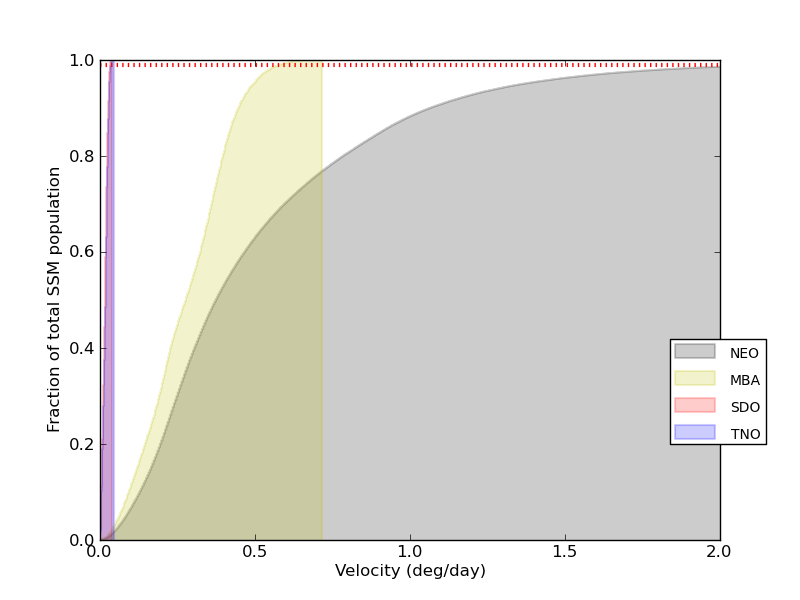
\includegraphics[width=13cm]{illustrations/mopsplots/aug2011/n_velocity.png}
  \caption{A cumulative histogram of solar solar system object
    sky-plane velocities, organized by classification.  Note that only
    the near-earth objects have higher velocities than main-belt
    asteroids.}
  \label{velSurvey}
\end{figure}

\begin{figure}[ht!]
  \centering
  \subfloat[Apparent Accelerations in Right Ascension over 15 Days]{
    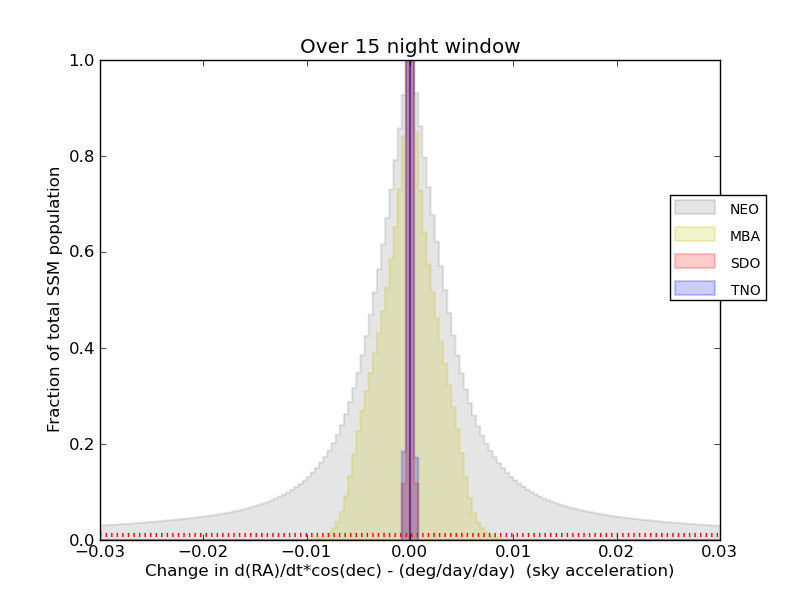
\includegraphics[width=8cm]{illustrations/mopsplots/aug2011/n_accel_ra_15.png}
    }
  \subfloat[Apparent Accelerations in Right Ascension over 30 Days]{
    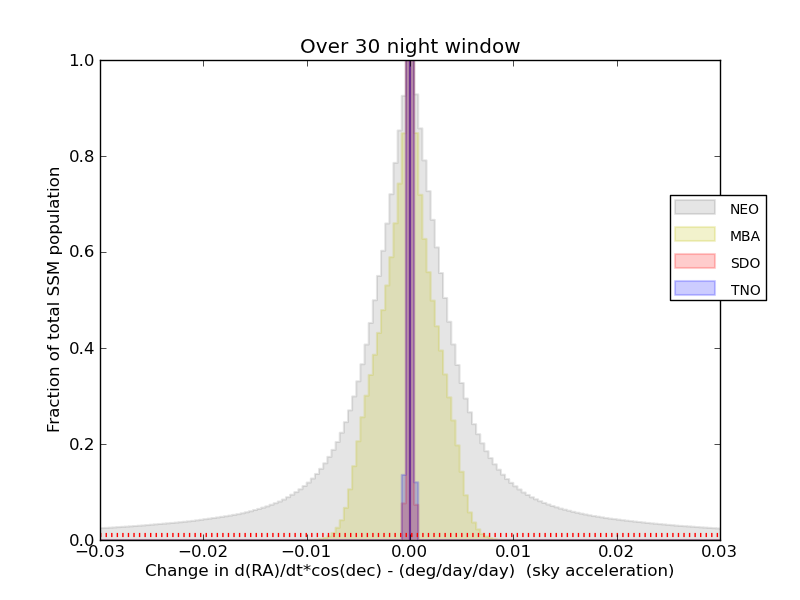
\includegraphics[width=8cm]{illustrations/mopsplots/aug2011/n_accel_ra_30.png}
    }

  \subfloat[Declination Apparent Accelerations in Declination over 15 Days]{
    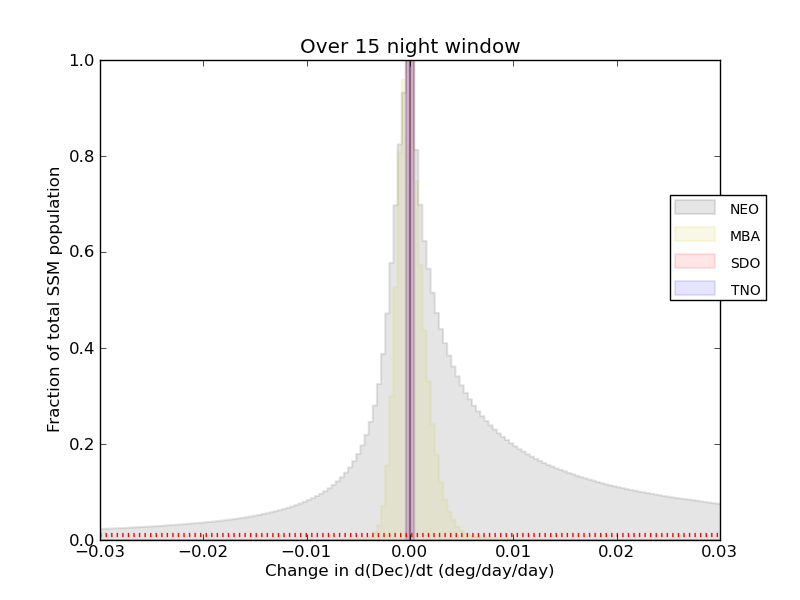
\includegraphics[width=8cm]{illustrations/mopsplots/aug2011/n_accel_dec_15.png}
    }
  \subfloat[Declination Apparent Accelerations in Declination over 30 Days]{
    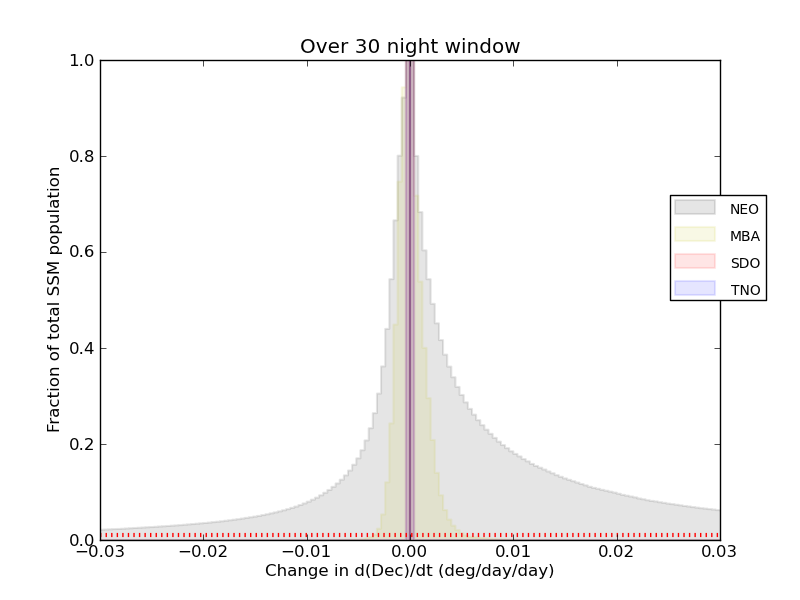
\includegraphics[width=8cm]{illustrations/mopsplots/aug2011/n_accel_dec_30.png}
    }
  \caption{Normalized histograms of sky-plane accelerations of several
    classes solar system objects in the RA and declination, with
    objects grouped by classification.  Histograms are presented for
    changes over 15 days and 30 days. The best-fit accelerations vary
    slightly given the size of the window; this is due to
    non-quadratic factors not included in the simple quadratic model.
    15 day tracking windows are used in the experiments presented in
    this document, but we expect to move to 30 day windows in the
    future.  In both cases, virtually all MBAs, and all other objects
    except NEOs, should have accelerations between -.02 and .02
    deg/day$^2$ in both axes.}
  \label{accSurvey}
\end{figure}


In order to determine reasonable limits on velocity and acceleration
of various classes of solar system objects, a survey of the solar
system model \citep{Grav2011} was conducted, see figures
\ref{velSurvey}, \ref{accSurvey} for histograms
presenting the results of these surveys.

We found that a velocity limit of .5 deg/day and an acceleration limit
.02 deg/day$^2$ would be generally sufficient.  By examining the
detections on an object-per-object basis, we calculated that among the
186,344 objects seen with proper cadence for OD, 186,209 of these
(more than 99.9\%) should generate useful tracks given these limits.

%% see mops64: /mnt/raid/jmyers/variousDensities/fullDensity/maxV.5_15days/trueTracks/*.log


\subsubsection{About the Simulated Source Catalog}
\label{sourceCatalog}
The simulated asteroid catalog was generated using the cadence of a
simulated survey conducted using the LSST Operations Simulator.  A set
of fields was chosen along the ecliptic: all fields with centers along
$(-8, 8)$ in RA and $(-7.4, 8)$ in declination were considered.  This
included images whose endpoints span a region of more than 367 square
degrees. For images of those fields, we generated ephemeris for
synthetic solar system objects which could appear in the image.  These
ephemerides were then filtered on location and magnitude based on the
filter and seeing of the images.  Astrometric error was added to these
ephemerides resulting in simulated DiaSources which were used as input
to the linking stages of MOPS.


\begin{figure}[ht!]
\centering
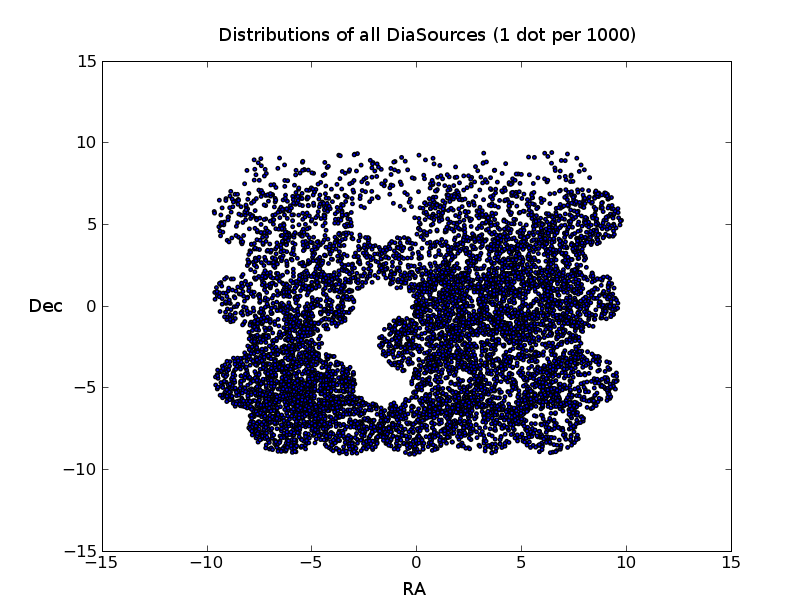
\includegraphics[scale=.7]{illustrations/allDias_1_1000th_density.png}
\caption{A reduced-density plot of simulated asteroid detections (DiaSources) used in our simulated catalog.  Detections from several fields were missing, but we expect that our results should be reasonably representative nonetheless.}
\label{diasPlot}
\end{figure}

A plot of some of the detections used in the simulation is presented
in figure \ref{diasPlot}.  As is visible in the plot, four of the
twenty-two fields had missing data due to a software error.  We expect
that the presence of this flaw in the data should not significantly
affect the conclusions reached from our experiments.



\subsection{Results}



\begin{figure}[ht!]
\centering \subfloat[Summary of results]{
\begin{tabular}{|r|r|}
%%%%%%%%%%%%%%%%%%%%%%%%%%%%%%%%%%%%%%%%%%%%%%%%%%%%%%%%%%%%%
\hline 
Tracklet generation runtime:  & 2,355 sec  (.6 hours) \\
Track generation runtime:     & 39,713 sec (11 hours) \\
Total linking runtime:        & 42,068 sec (11.7 hours) \\
Peak memory usage:            & 2.2 GB \\
 & \\
Number of tracklets:          & 4,502,224  \\
Tracklet \% true:             & 43.4\% \\
Number of tracks:             & 3,318,539 \\
Track \% true:                & 26.6\% \\
 & \\
Estimated OD cost (assuming 1000 OD/sec):  & 3,318 sec (.9 hours) \\
Estimated total resource usage:      & 45,386 sec (12.6 hours)\\
 & \\
Number of findable objects:   & 186,344 \\
Number of objects found:      & 176,080 \\
\% Found / findable:          & 94.5\% \\
\hline
%%%%%%%%%%%%%%%%%%%%%%%%%%%%%%%%%%%%%%%%%%%%%%%%%%%%%%%%%%%%%
\end{tabular}
}

\subfloat[Found objects by type]{
\begin{tabular}{|r|r|r|r|}
\hline
Object class            & Number found & Number findable & Percent found/findable \\
\hline
Main-belt objects       & 172,539   &  182,285     & 94.7\%  \\
Near-earth objects      & 276       &  504         & 54.8\%        \\
Comets                  & 1,374     &  1,534       & 89.6\%      \\
Trojans                 & 1,593     &  1,696       & 93.9\%      \\
Trans-Neptunian objects & 254       &   281        & 90.4\%      \\
Scattered disk objects  & 44        &    44        & 100\%       \\
\hline
\end{tabular}
}

\caption{In-depth results from our simulated survey of full-density asteroid sources from a subset of the visible sky.}
\label{bigSimResults}
\end{figure}

Our simulated survey was run using a single 2.2 GHz Opteron core.
Results from our simulated survey are presented in figure
\ref{bigSimResults}.  Our success rate for discovery of findable
objects was quite high (just below 95\%) and the number of tracks
generated was reasonably small, meaning that running OD on the output
should not be computationally expensive.  This is a significant
difference from the experiences reported by the PanSTARRS MOPS, in
which OD is considered to be the most expensive phase of processing.
This is because the PanSTARRS MOPS uses a more permissive RMS filter
where our simulation used a less permissive chi-squared
probability-based filter, greatly reducing the number of false tracks.

We also present the types of objects found by class; though our
filters were tuned for main-belt objects, we had a high rate of
success in finding several other types of objects.  Near-earth objects
were underrepresented due to their high velocities; see
\ref{neosTrailing} for future plans to address this.



\subsection{Scaling On Solar System Model Density}

To test the scaling of the system as density increases, we generated
``reduced-density'' catalogs.  We randomly chose a subset of the
objects observed in the original catalog and removed all detections of
those objects, then ran DayMOPS on the resulting catalog.  We found
that our software continued to find nearly all the remaining findable
objects regardless of density, though the linking runtimes increased
significantly as density increased. See figure \ref{ssmDensity} for
results.


\begin{figure}
\centering
\subfloat{
\footnotesize
\begin{tabular}{|c|r|r|r|r|r|r|}
  \hline 
  SSM Density & \#DiaSources & \#Tracklets & \#Tracks & Linking Runtime (sec) & Track \% True & Found/Findable   \\
  \hline
  .1        & 827021  &   211,635    & 122,160   & 669         & 75.97\%  & 95.31\% \\
  .025      & 2070722 &   649,907    & 401,895   & 3,664        & 57.94\%  & 94.71\% \\
  .05       & 4140278 & 1,618,205    & 1,116,346 & 17,304       & 40.70\%  & 94.91\% \\
  .75       & 6197009 & 2,897,291    & 2,085,296 & 46,077       & 32.14\%  & 94.74\% \\
  1.0       & 8274898 & 4,502,224    & 3,318,420 & 98,848       & 26.61\%  & 94.56\% \\
  \hline
\end{tabular}
}







\subfloat{
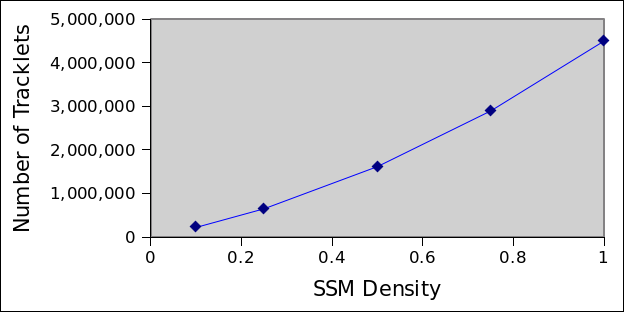
\includegraphics[scale=.4]{illustrations/density_v_nTracklets.png}
}
\subfloat{
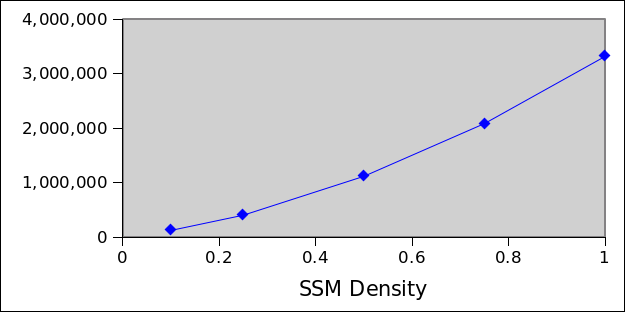
\includegraphics[scale=.4]{illustrations/density_v_nTracks.png}
}


\subfloat{
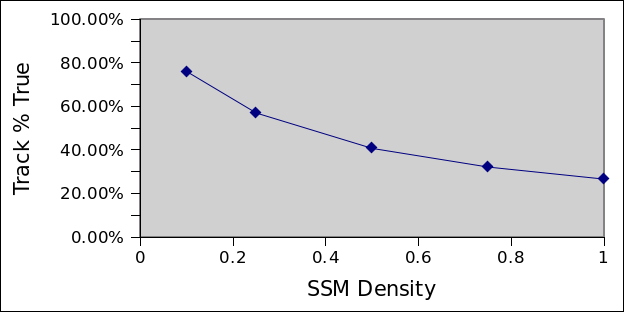
\includegraphics[scale=.4]{illustrations/density_v_trackTrue.png}
}
\subfloat{
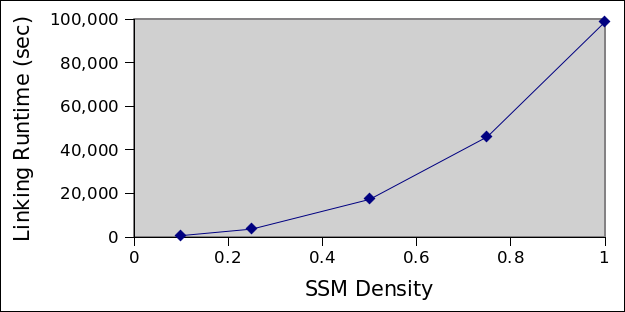
\includegraphics[scale=.4]{illustrations/density_v_runtime.png}
}


\caption{ Results from running DayMOPS linking methods on reduced-density source catalogs. }

\label{ssmDensity}

\end{figure}














\subsection{Scaling On Non-Solar System Detection Density}

Even after removal of background stars, actual observational data will
include a variety of non-asteroid sources, including transient
phenomena and image processing artifacts.  In order to estimate the
tolerance of DayMOPS linking methods to these sources, we carried out
a series of simulated surveys which included varying numbers of
randomly-distributed ``noise'' sources throughout each simulated
image.  To reduce the runtime of the experiment, the asteroid
detection catalog was taken from the 50\%-density SSM catalog from the
prior experiment.  The addition of noise had little impact on the
ability of the software to find nearly all the findable objects, but
did result in increased runtime for the linking phase.  See figure
\ref{noiseDensity} for results.





\begin{figure}

\subfloat{
\footnotesize
\begin{tabular}{|r|r|r|r|r|r|r|}
  \hline 
Noise Points / Image &   \% Noise & \#Tracklets & \#Tracks  & Linking Runtime (sec) & Track \% True & Found/Findable \\
0      &     0.0\%    &  1,618,205  & 1,116,346 & 8,413           &  40.70\%      &  94.91\%       \\
500    &     20.63\%  & 1,947,235   & 1,127,355 & 9,996           & 40.28\%       &  94.90\%       \\
2,500  &     56.51\%  & 4,107,233   & 1,202,270 & 19,321          & 50.36\%       &  94.87\%       \\
5,000  &     72.21\%  & 8,693,128   & 1,361,796 & 51,008          & 33.14\%       &  94.80\%       \\
10,000 &     83.87\%  & 23,989,975  & 1,951,794 & 256,565         & 22.89\%       &  94.62\%       \\
   \hline
\end{tabular}
}

\subfloat{
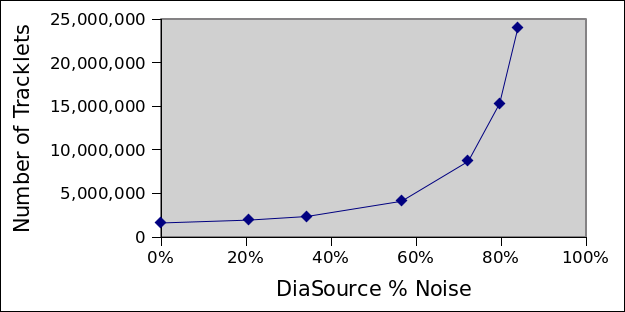
\includegraphics[scale=.4]{illustrations/noise_v_nTracklets.png}
}
\subfloat{
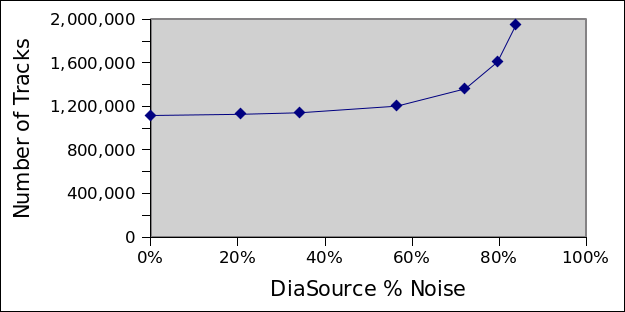
\includegraphics[scale=.4]{illustrations/noise_v_nTracks.png}
}

\subfloat{
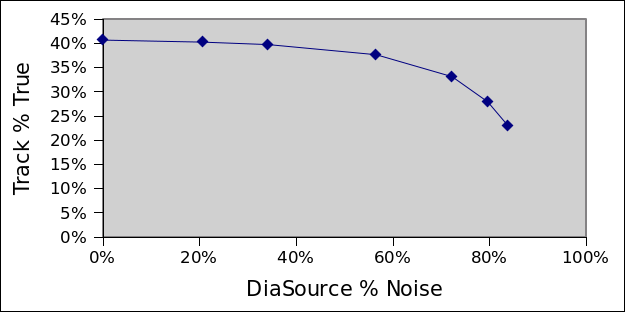
\includegraphics[scale=.4]{illustrations/noise_v_trackTrue.png}
}
\subfloat{
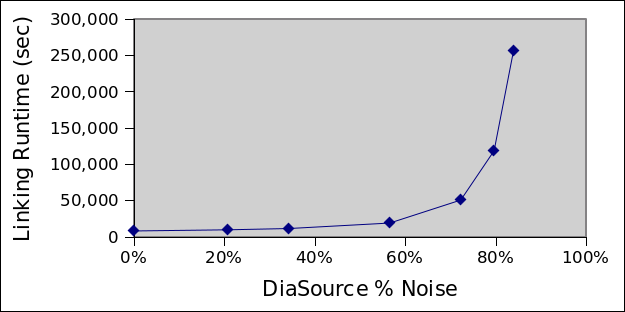
\includegraphics[scale=.4]{illustrations/noise_v_runtime.png}
}

\caption{Results from a simulated survey using a 50\%-density SSM and
  varying numbers of randomly-distributed ``noise'' (non-asteroid)
  sources per image.}
\label{noiseDensity}
\end{figure}





